\documentclass{article}[12pt]
\usepackage{fullpage,graphicx, setspace, latexsym, cite,amsmath,amssymb,color,subfigure}
%\usepackage{epstopdf}
%\DeclareGraphicsExtensions{.pdf,.eps,.png,.jpg,.mps} 

\let\proof\relax
\let\endproof\relax
\let\example\relax
\let\endexample\relax

\usepackage{amssymb} %maths
\usepackage{amsmath} %maths
\usepackage{amsthm}
\usepackage{float}

\bibliographystyle{unsrt}

\newtheorem{theorem}{Theorem}
\newtheorem{prop}{Proposition}
\newtheorem{corollary}{Corollary}
\newtheorem{lemma}{Lemma}
\newtheorem{remark}{Remark}
\newtheorem{defn}{Definition}
\newtheorem{ex}{Example}
\usepackage{float}

\def\R{\mathbb{R}}
\def\Eps{\mathcal{E}}
\def\E{\mathbb{E}}
\def\V{\mathbb{V}}
\def\F{\mathcal{F}}
\def\G{\mathcal{G}}
\def\H{\mathcal{H}}
\def\S{\mathcal{S}}
\def\P{\mathbb{P}}
\def\1{\mathbf{1}}
\def\n{\nappa}
\def\h{\mathbf{w}}
\def\v{\mathbf{v}}
\def\x{\mathbf{x}}
\def\X{\mathcal{X}}
\def\Y{\mathcal{Y}}
\def\eps{\epsilon}
\def\y{\mathbf{y}}
\def\e{\mathbf{e}}
\newcommand{\norm}[1]{\left|\left|#1\right|\right|}
\DeclareMathOperator*{\argmin}{arg\,min}
\DeclareMathOperator*{\argmax}{arg\,max}

\newcommand{\lecture}[4]{
   \pagestyle{myheadings}
   \thispagestyle{plain}
   \newpage
   % \setcounter{lecnum}{#1}
   \setcounter{page}{1}
   \setlength{\headsep}{10mm}
   \noindent
   \begin{center}
   \framebox{
      \vbox{\vspace{2mm}
    \hbox to 6.28in { {\bf ESE 680-004: Learning and Control
   \hfill Fall 2019} }
       \vspace{4mm}
       \hbox to 6.28in { {\Large \hfill Lecture #1: #2  \hfill} }
       \vspace{2mm}
       \hbox to 6.28in { {\it Lecturer: #3 \hfill Scribes: #4} }
      \vspace{2mm}}
   }
   \end{center}
   \markboth{Lecture #1: #2}{Lecture #1: #2}

   \noindent{\bf Disclaimer}: {\it These notes have not been subjected to the
   usual scrutiny reserved for formal publications. }
   \vspace*{4mm}
}

%notation

\def \E{\mathbb E}
\def \P{\mathbb P}
\def \R{\mathbb R}
\def \A{\cal A}

\begin{document}

\lecture{11}{System Level Synthesis and Robust Control Bounds}{Nikolai Matni}{Haimin Hu}

\section{Introduction}

In the last few lectures we have seen how to use machine learning and probability tools to perform system identification and quantify associated uncertainties. More specifically, these uncertainties are produced via concentration bounds and they are in form of error bounds with probability profiles. Now, as depicted in Figure \ref{fig::1}, the remaining component in our familiar learning and control pipeline is, how do we explicitly account for this uncertainty when designing control policies?
In this lecture, we will see ways to handle uncertainties stemming from system identification using robust control tools. In the end, we would expect end-to-end guarantees like:

\vspace{0.2cm}
\noindent \textit{With probability $1-\delta$, for $N$ sufficiently large, the synthesized
controller is stabilizing and achieves the relative performance bound}
\begin{equation}
\label{end_to_end}
    \frac{\hat{J}-J_{\star}}{j_{\star}} \leq C(\text { robustness, excitability }) \sqrt{\frac{(d+p) \log \left(\frac{1}{\delta}\right)}{N}}
\end{equation}
where $\hat{J}$ is the performance of the learned controller on true system, $J_\star$ is the optimal performance achievable, $d$ is the number of states and $p$ is the number of inputs. Further notice that $C$ is a constant depending only on the true system matrices.


\begin{figure}[H]
    \centering
    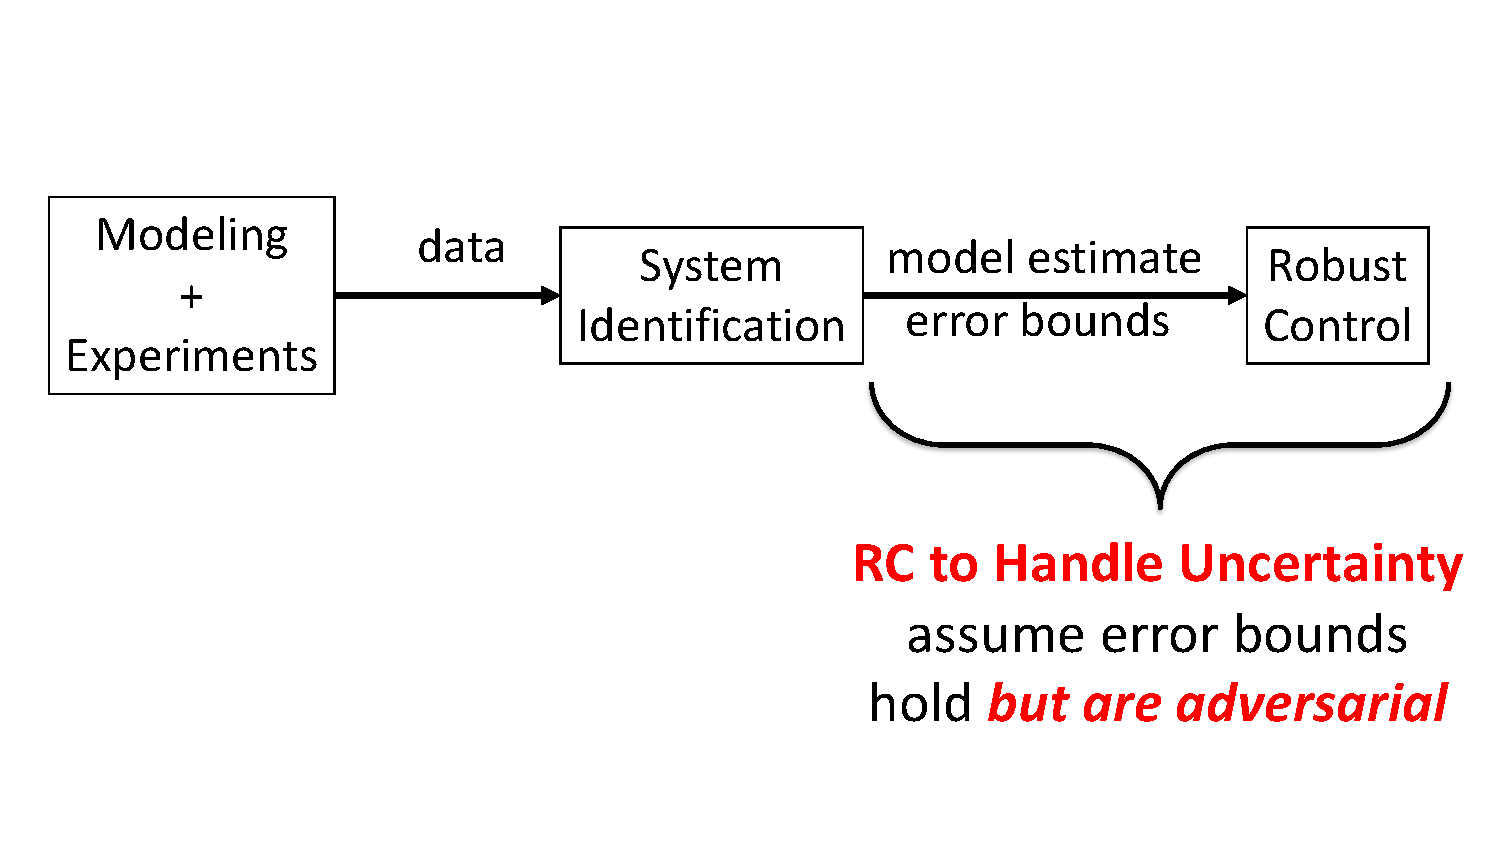
\includegraphics[width=0.5\linewidth]{1.pdf}
    \caption{\label{fig::1} A learning and control pipeline}
\end{figure}

Denote $\Delta A = \hat{A} - A$ and $\Delta B = \hat{B} - B$, the uncertainties in estimated system matrices. If we know that $|| \Delta_{A}|| \leq \varepsilon_{A}, ||  \Delta_{B}|| \leq \varepsilon_{B}$, the main challenge therein is to quantify the performance degradation of a robust controller with respect to the optimal controller as a function of $\left(\varepsilon_{A}, \varepsilon_{B}\right)$. We will see that \textit{System Level Synthesis} (SLS) is an effective way to achieve robust control synthesis in this context.

\section{Finite Horizon System Level Synthesis}
Consider the linear time varying (LTV) system
\begin{equation}
    \label{eq::LTV}
    x_{t+1}=A_{t} x_{t}+B_{t} u_{t}+w_{t}
\end{equation}
where $x_{t} \in \mathbb{R}^{n} \text { is the state, } u_{t} \in \mathbb{R}^{p} \text { is the control input and } w_{t} \in \mathbb{R}^{n} \text { is the disturbance}$. We consider a time horizon of $t=0, \ldots, T$.
Let us define a linear and time-varying state-feedback law in form of
\begin{equation}
    \label{eq::control_law}
    u_{t}=\sum_{\tau=0}^{t} K_{t, t-\tau} x_{\tau}
\end{equation}
and write the signals in compact form
\begin{equation}
\label{eq::BLT}
    \mathbf{x}=\left[\begin{array}{c}{x_{0}} \\ {x_{1}} \\ {\vdots} \\ {x_{T}}\end{array}\right], \mathbf{u}=\left[\begin{array}{c}{u_{0}} \\ {u_{1}} \\ {\vdots} \\ {u_{T}}\end{array}\right] \quad \mathbf{w}=\left[\begin{array}{c}{x_{0}} \\ {w_{0}} \\ {w_{1}} \\ {\vdots} \\ {w_{T-1}}\end{array}\right], \mathbf{K}=\left[\begin{array}{cccc}{K^{0,0}} & {} & {} & {} \\ {K^{1,1}} & {K^{1,0}} & {} & {} \\ {\vdots} & {\ddots} & {\ddots} & {} \\ {K^{T, T}} & {\ldots} & {K^{T, 1}} & {K^{T, 0}}\end{array}\right]
\end{equation}
Now, we introduce down-shift operator $Z$, i.e. a matrix with identity matrices along the first block sub-diagonal and zeros elsewhere. Subsequently, we can compactly rewrite the behavior of the system \eqref{eq::LTV} as
\begin{equation}
\label{eq::close_loop_behav}
    \begin{array}{l}{\mathbf{x}=(I-Z(\mathcal{A}+\mathcal{B}\mathbf{K}))^{-1} \mathbf{w}} \\ {\mathbf{u}=\mathbf{K}(I-Z(\mathcal{A}+\mathcal{B}\mathbf{K}))^{-1} \mathbf{w}}\end{array}
\end{equation}
where $\mathcal{A}:=\text { blkdiag }\left(A_{0}, A_{1}, \ldots, A_{T-1}, 0\right), \mathcal{B}:=\operatorname{blkdiag}\left(B_{0}, B_{1}, \ldots, B_{T-1}, 0\right)$.
In other words, these maps describe the system responses achieved by feedback law $\mathbf{K}$
from $\mathbf{w}$ to $(\mathbf{x},\mathbf{u})$.
Here, we highlight that the key idea of SLS is to optimize directly over those maps, as opposed to $\mathbf{K}$. More concretely, we would like to optimize over Block Lower Triangular (BLT) matrices $\left\{\mathbf{\Phi}_{x}, \mathbf{\Phi}\right\}$ defined as
\begin{equation}
    \mathbf{\Phi}_{x}=\left[\begin{array}{cccc}{\Phi_{x}^{0,0}} & {} & {} & {} \\ {\Phi_{x}^{1,1}} & {\Phi_{x}^{1,0}} & {} & {} \\ {\vdots} & {\ddots} & {\ddots} & {} \\ {\Phi_{x}^{T, T}} & {\cdots} & {\Phi_{x}^{T, 1}} & {\Phi_{x}^{T, 0}}\end{array}\right], \mathbf{\Phi}_{u}=\left[\begin{array}{cccc}{\Phi_{u}^{0,0}} & {} & {} & {} \\ {\Phi_{u}^{1,1}} & {\Phi_{u}^{1,0}} & {} & {} \\ {\vdots} & {\ddots} & {\ddots} & {} \\ {\Phi_{u}^{T, T}} & {\cdots} & {\Phi_{u}^{T, 1}} & {\Phi_{u}^{T, 0}}\end{array}\right]
\end{equation}
and they satisfy
\begin{equation}
\label{eq::behav}
    \left[\begin{array}{l}{\mathbf{x}} \\ {\mathbf{u}}\end{array}\right]=\left[\begin{array}{l}{\mathbf{\Phi}_{x}} \\ {\mathbf{\Phi}_{u}}\end{array}\right] \mathbf{w}
\end{equation}
The following theorem ensures that there exists a BLT controller $\mathbf{K}$ such that the closed loop system \eqref{eq::close_loop_behav} achieves the desired behavior \eqref{eq::behav}.

\begin{theorem}[Theorem 2.1 \cite{anderson2019system}]
\label{thm::achieve}
For the dynamics \eqref{eq::LTV} over a horizon $t=0, \dots, T,$ for BLT $\mathbf{K}$ and $\mathbf{u}=\mathbf{K} \mathbf{x}$, the following are equivalent:
\begin{enumerate}
    \item The affine space of BLT $(\mathbf{\Phi}_{x}, \mathbf{\Phi}_u)$ satisfying 
    \begin{equation}
    \label{eq::affine_constr}
        \left[\begin{array}{cc}{I-Z \mathcal{A}} & {-Z \mathcal{B}}\end{array}\right]\left[\begin{array}{c}{\boldsymbol{\Phi}_{x}} \\ {\mathbf{\Phi}_{u}}\end{array}\right]=I
    \end{equation}
    parameterizes all achievable maps \eqref{eq::behav}.
    \item For all $(\mathbf{\Phi}_{x}, \mathbf{\Phi}_u)$ satisfying the above constraint, denoted by $\mathcal{C}\left(\mathbf{\Phi}_{x}, \mathbf{\Phi}_{u}\right)=I$ for short, the controller $\mathbf{K}=\mathbf{\Phi}_{u} \mathbf{\Phi}_{x}^{-1}$ achieves the desired response \eqref{eq::behav}.
\end{enumerate}
\end{theorem}

\begin{proof}
$1 \Rightarrow 2$: Notice first that $\mathbf{\Phi}^{-1}_x$ exists because \eqref{eq::affine_constr} implies that its block-diagonal components are $I$. By substituting $\mathbf{K}=\mathbf{\Phi}_{u} \mathbf{\Phi}_{x}^{-1}$ into \eqref{eq::close_loop_behav} we have that
\begin{equation}
    \mathbf{x}=\left(I-Z\left(\mathcal{A}+\mathcal{B} \mathbf{\Phi}_{u} \mathbf{\Phi}_{x}^{-1}\right)\right)^{-1} \mathbf{w}
\end{equation}
Consider the following algebra
\begin{equation}
    \left.\left(I-Z\left(\mathcal{A}+\mathcal{B} \mathbf{\Phi}_{u} \mathbf{\Phi}_{x}^{-1}\right)\right)^{-1}=\left((I-Z \mathcal{A}) \mathbf{\Phi}_{x}-Z \mathcal{B} \mathbf{\Phi}_{u}\right) \mathbf{\Phi}_{x}^{-1}\right)^{-1}=\mathbf{\Phi}_{x}\left((I-Z \mathcal{A}) \mathbf{\Phi}_{\mathbf{x}}-Z \mathcal{B} \mathbf{\Phi}_{u}\right)^{-1}=\mathbf{\Phi}_{x}
\end{equation}
the last step is implied by 1. For the control map:
\begin{equation}
    \mathbf{u}=\mathbf{\Phi}_{u} \mathbf{\Phi}_{x}^{-1} \mathbf{x}=\mathbf{\Phi}_{u} \mathbf{\Phi}_{x}^{-1} \mathbf{\Phi}_{x} \mathbf{w}=\mathbf{\Phi}_{u} \mathbf{w}
\end{equation}

\noindent $2 \Rightarrow 1$: Consider the following algebra
\begin{equation}
    [I-Z \mathcal{A} \ -Z \mathcal{B}]\left[\begin{array}{c}{(I-Z(\mathcal{A}+\mathcal{B} \mathbf{K}))^{-1}} \\ {\mathbf{K}(I-Z(\mathcal{A}+\mathcal{B }\mathbf{K}))^{-1}}\end{array}\right]=(I-Z \mathcal{A}-Z \mathcal{B} \mathbf{K})(I-Z(\mathcal{A}+\mathcal{B} \mathbf{K}))^{-1}=I
\end{equation}
where we have utilized the definition of $(\mathbf{\Phi}_{x}, \mathbf{\Phi}_u)$ via \eqref{eq::close_loop_behav}.
\end{proof}

\subsection{Recipe of Formulating SLS Problems}
To summarize, there are three steps for turning a standard finite-time optimal control problem (FTOCP) into an SLS problem:
\begin{enumerate}
    \item Rewrite the problem in vector + BLT notation \eqref{eq::BLT}.
    \item Set $\mathbf{x}=\mathbf{\Phi}_{x} \mathbf{w}, \text { and } \mathbf{u}=\mathbf{\Phi}_{u} \mathbf{w}$ and constrain $(\mathbf{\Phi}_{x}, \mathbf{\Phi}_u)$ to obey $\mathcal{C}\left(\mathbf{\Phi}_{x}, \mathbf{\Phi}_{u}\right)=I$.
    \item Optimize over system responses $(\mathbf{\Phi}_{x}, \mathbf{\Phi}_u)$ with appropriate disturbance model and cost function.
\end{enumerate}
In the following we perform those steps on LQR and $\mathcal{L}_1$ optimal control as illustrative examples.

\subsection{Constrained LQR without Noise}
The finite-time constrained LQR problem is formulated as
\begin{equation}
\label{LQR}
    \begin{aligned} \min _{x_{t}, u_{t}} & \sum_{t=0}^{T} x_{t}^{\top} Q_{t} x_{t}+u_{t}^{\top} R_{t} u_{t} \\ \text { subject to } & x_{t+1}=A x_{t}+B u_{t}, \ t=0, \ldots, T-1 \\ & x_{0} \text { known } \\ & x_{t} \in \mathcal{X}_{t}, u_{t} \in \mathcal{U}_{t} \end{aligned}
\end{equation}
Using vector notation, this problem can be written as
\begin{equation}
\label{LQR::vec}
    \begin{aligned} \min _{\mathbf{x}, \mathbf{u}} &\left\|\left[\begin{array}{cc}{\mathcal{Q}^{\frac{1}{2}}} & {0} \\ {0} & {\mathcal{R}^{\frac{1}{2}}}\end{array}\right]\left[\begin{array}{l}{\mathbf{x}} \\ {\mathbf{u}}\end{array}\right]\right\|_{F}^{2} \\ \text { subject to } & \mathbf{x}=Z \mathcal{A} \mathbf{x}+Z \mathcal{B} \mathbf{u} \\ & \boldsymbol{x} \in \mathcal{X}, \mathbf{u} \in \mathcal{U} \end{aligned}
\end{equation}
where $\mathbf{w}=\left[x_0^\top \ 0 \ \ldots \ 0 \right]^\top$, $\mathcal{Q}:=\text {blkdiag}\left(Q_{0}, Q_{1}, \ldots, Q_{T}\right)$ and $\mathcal{R}:=\text {blkdiag}\left(R_{0}, R_{1}, \ldots, R_{T}\right)$.
Notice that $\mathbf{x}=\mathbf{\Phi}_{x} \mathbf{w}=\mathbf{\Phi}_{x}(:, 0) x_{0} \text { and } \mathbf{u}=\mathbf{\Phi}_{u} \mathbf{w}=\mathbf{\Phi}_{u}(:, 0) x_{0}$. Here we use $\mathbf{\Phi}(:, 0)$ to denote the first block column of a matrix $\mathbf{\Phi}$. Applying Theorem \ref{thm::achieve} to \eqref{LQR::vec} we arrive at
\begin{equation}
    \begin{array}{c}{\min _{\Phi_{x}, \Phi_{u}}\left\|\left[\begin{array}{cc}{\mathcal{Q}^{\frac{1}{2}}} & {0} \\ {0} & {\mathcal{R}^{\frac{1}{2}}}\end{array}\right]\left[\begin{array}{l}{\mathbf{\Phi}_{x}(:, 0)} \\ {\mathbf{\Phi}_{u}(:, 0)}\end{array}\right] x_{0}\right\|_{F}^{2}} \\ {\text { subject to }[I-Z \mathcal{A}-Z \mathcal{B}]\left[\begin{array}{l}{\mathbf{\Phi}_{x}(:, 0)} \\ {\mathbf{\Phi}_{u}(:, 0)}\end{array}\right]=I} \\ \qquad \qquad \  {\mathbf{\Phi}_{x}(:, 0) x_{0} \in \mathcal{X}, \ \mathbf{\Phi}_{u}(:, 0) x_{0} \in \mathcal{U}}\end{array}
\end{equation}
This is an SDP problem which can be solved efficiently using existing solvers, for example \texttt{MOSEK}.

\subsection{$\mathcal{L}_1$ Optimal Control}
Consider the following $\mathcal{L}_1$ optimal control in vector form
\begin{equation}
    \begin{array}{c}{\min _{\mathbf{x}, \mathbf{u}} \max _{\|\mathbf{w}\|_{\infty} \leq 1}\left\|\left[\begin{array}{cc}{\mathcal{Q}^{\frac{1}{2}}} & {0} \\ {0} & {\mathcal{R}^{\frac{1}{2}}}\end{array}\right]\left[\begin{array}{c}{\mathbf{x}} \\ {\mathbf{u}}\end{array}\right]  \right\|_{\infty}} \\ {\text { subject to } \qquad \ \mathbf{x}=Z \mathcal{A} \mathbf{x}+Z \mathcal{B} \mathbf{u}+\mathbf{w}}\end{array}
\end{equation}
Once again we apply Theorem \ref{thm::achieve} and arrive at
\begin{equation}
    \begin{array}{c}{\min _{\mathbf{\Phi}_{x}, \mathbf{\Phi}_{u}} \max _{\|\mathbf{w}\|_{\infty} \leq 1}\left\|\left[\begin{array}{cc}{\mathcal{Q}^{\frac{1}{2}}} & {0} \\ {0} & {\mathcal{R}^{\frac{1}{2}}}\end{array}\right]\left[\begin{array}{c}{\mathbf{\Phi}_{x}} \\ {\mathbf{\Phi}_{u}}\end{array}\right] \mathbf{w} \right\|_{\infty}} \\ {\text { subject to } \qquad \qquad [I-Z \mathcal{A} \ -Z \mathcal{B}]\left[\begin{array}{c}{\mathbf{\Phi}_{x}} \\ {\mathbf{\Phi}_{u}}\end{array}\right]=I}\end{array}
\end{equation}
Using the definition of $\mathcal{L}_1$ norm we can eliminate the inner optimization problem over $\mathbf{w}$, leading to the
final optimization problem over system responses $(\mathbf{\Phi}_{x}, \mathbf{\Phi}_u)$
\begin{equation}
    \begin{array}{c}{\min _{\mathbf{\Phi}_{x}, \mathbf{\Phi}_{u}} \left\|\left[\begin{array}{cc}{\mathcal{Q}^{\frac{1}{2}}} & {0} \\ {0} & {\mathcal{R}^{\frac{1}{2}}}\end{array}\right]\left[\begin{array}{c}{\mathbf{\Phi}_{x}} \\ {\mathbf{\Phi}_{u}}\end{array}\right]  \right\|_{\infty \rightarrow \infty}} \\[0.3cm] {\text { subject to } \  [I-Z \mathcal{A} \ -Z \mathcal{B}]\left[\begin{array}{c}{\mathbf{\Phi}_{x}} \\ {\mathbf{\Phi}_{u}}\end{array}\right]=I}\end{array}
\end{equation}
Notice that this is a linear program and thus can be solved efficiently.


\section{Infinite-Horizon State-Feedback SLS}
Now, let us try to extend results on finite-horizon SLS in Section 2 to the setting of infinite-horizon optimal control. Consider a linear time invariant (LTI) plant
\begin{equation}
\label{LTI}
    x(t+1)=A x(t)+B u(t)+ B_w w(t)
\end{equation}
The $z$-transform of dynamics \eqref{LTI} is given by
\begin{equation}
    (z I-A) \mathbf{x}=B \mathbf{u}+\boldsymbol{\delta}_{\boldsymbol{x}}
\end{equation}
where $\boldsymbol{\delta}_{\boldsymbol{x}}:=B_{w} \mathbf{w}$ denote the disturbance affecting the state.
Consider state-feedback control policy $\mathbf{u}=\mathbf{K x}$ as defined in \eqref{eq::control_law} and substitute it into the above equation, leading to system responses $(\mathbf{\Phi}_{x}, \mathbf{\Phi}_u)$ for \eqref{LTI} defined as 
\begin{equation}
\label{map::inf}
    \begin{aligned} \mathbf{\Phi}_{x} &=\left(z I-A-B \mathbf{K}\right)^{-1} \\ \mathbf{\Phi}_{u} &=\mathbf{K}\left(z I-A-B \mathbf{K}\right)^{-1} \end{aligned}
\end{equation}

\begin{theorem}[Theorem 4.1 \cite{anderson2019system}]
\label{thm::achieve_inf}
For the LTI dynamics \eqref{LTI} under state-feedback control law $\mathbf{u}=\mathbf{K} \mathbf{x}$, the following statements are equivalent:
\begin{enumerate}
    \item The affine space of BLT $(\mathbf{\Phi}_{x}, \mathbf{\Phi}_u)$ satisfying 
    \begin{equation}
    \label{eq::affine_constr_inf}
        \left[\begin{array}{cc}{z I-A} & {-B}\end{array}\right]\left[\begin{array}{c}{\mathbf{\Phi}_{x}} \\ {\mathbf{\Phi}_{u}}\end{array}\right]=I, \quad \mathbf{\Phi}_{x}, \mathbf{\Phi}_{u} \in \frac{1}{z}  \mathcal{RH}_{\infty}
    \end{equation}
    parameterizes all responses \eqref{map::inf}, achievable by an
    internally stabilizing state feedback controller $\mathbf{K}$.
    \item For all $(\mathbf{\Phi}_{x}, \mathbf{\Phi}_u)$ satisfying \eqref{eq::affine_constr_inf}, the controller $\mathbf{K}=\mathbf{\Phi}_{u} \mathbf{\Phi}_{x}^{-1}$, implemented as
    \begin{equation}
    \label{contrl::inf}
        \begin{aligned} \mathbf{u} &=z \Phi_{u} \hat{\delta}_{x} \\ \hat{\delta}_{x} &=\mathbf{x}+\left(I-z \Phi_{x}\right) \hat{\delta}_{x} \end{aligned}
    \end{equation}
    is internally stabilizing and achieves the desired response \eqref{map::inf}.
\end{enumerate}
\end{theorem}

\begin{proof}
Almost identical to Theorem \ref{thm::achieve}. See Section 4 in \cite{anderson2019system}.
\end{proof}

\begin{remark}
Constraint $\mathbf{\Phi}_{x}, \mathbf{\Phi}_{u} \in \frac{1}{z}  \mathcal{RH}_{\infty}$ in \eqref{eq::affine_constr_inf} means that systems responses $(\mathbf{\Phi}_{x}, \mathbf{\Phi}_u)$ are stable and strictly proper.
\end{remark}


\section{Robust SLS}
In this section, we will develop robustness result for the infinite-horizon SLS that
provides necessary and sufficient conditions under which a controller that only approximately satisfies the achievability constraint \eqref{eq::affine_constr_inf} is stabilizing.


\subsection{Robust Achievability and Stability}
Let us now derive the robust variant of Theorem \ref{thm::achieve_inf}, which shows achievability and stability for the infinite-horizon SLS under the presence of uncertainty.
\begin{theorem}[Theorem 4.3 \cite{anderson2019system}]
\label{thm::achieve::robust}
Let $\left(\hat{\mathbf{\Phi}}_{x}, \hat{\mathbf{\Phi}}_{u}, \mathbf{\Delta}\right)$ be a solution to
\begin{equation}
\label{achieve::robust}
    \left[\begin{array}{cc}{z I-A} & {-B}\end{array}\right]\left[\begin{array}{c}{\hat{\mathbf{\Phi}}_{x}} \\ {\hat{\mathbf{\Phi}}_{u}}\end{array}\right]=I+\mathbf{\Delta}, \quad \hat{\mathbf{\Phi}}_{x}, \hat{\mathbf{\Phi}}_{u} \in \frac{1}{z} \mathcal{R} \mathcal{H}_{\infty}
\end{equation}
and assume that $(I-\mathbf{\Delta})^{-1}$ exists. Then the controller $\boldsymbol{K}=\hat{\boldsymbol{\Phi}}_{u} \hat{\mathbf{\Phi}}_{x}^{-1}$ achieves the response
\begin{equation}
    \left[\begin{array}{l}{\boldsymbol{x}} \\ {\boldsymbol{u}}\end{array}\right]=\left[\begin{array}{l}{\hat{\boldsymbol{\Phi}}_{x}} \\ {\hat{\boldsymbol{\Phi}}_{u}}\end{array}\right](I-\boldsymbol{\Delta})^{-1} \boldsymbol{w}
\end{equation}
Further, $\mathbf{K} \text { is stabilizing if and only if }(I-\Delta)^{-1} \in \mathcal{R} \mathcal{H}_{\infty}$.
\end{theorem}

\begin{proof}
First multiply $(I-\mathbf{\Delta})^{-1}$ to both sides of \eqref{achieve::robust} and we have
\begin{equation}
    \left[\begin{array}{cc}{z I-A} & {-B}\end{array}\right]\left[\begin{array}{c}{\hat{\mathbf{\Phi}}_{x}} \\ {\hat{\mathbf{\Phi}}_{u}}\end{array}\right] (I-\mathbf{\Delta})^{-1} = I
\end{equation}
Then follow proof of Theorem \ref{thm::achieve_inf}. For the control we have that
\begin{equation}
    \mathbf{u} = \hat{\mathbf{\Phi}}_{u} (I-\mathbf{\Delta})^{-1}  \left[ \hat{\mathbf{\Phi}}_{x} (I-\mathbf{\Delta})^{-1} \right]^{-1} = \hat{\mathbf{\Phi}}_{u} \hat{\mathbf{\Phi}}_{x}^{-1} \mathbf{x} = \mathbf{K} \mathbf{x}
\end{equation}
Finally, to show that $\mathbf{K}$ is stabilizing refer to Section 4.5.1 in \cite{anderson2019system}.
\end{proof}

\subsection{Robust LQR Synthesis}
Now we would like to understand how our model error in system matrices $(A,B)$ affects closed loop behavior and performance. Recall the following assumption on the model uncertainty
\begin{equation}
\label{uncertainty}
\Delta_{A}:=\widehat{A}-A, \quad \Delta_{B}:=\widehat{B}-B, \quad \max \left\{\left\|\Delta_{A}\right\|,\left\|\Delta_{B}\right\|\right\} \leq \epsilon
\end{equation}
Let the noise term $w(t)$ in \eqref{LTI} be such that $w(t) := w_t \stackrel{i . i . d}{\sim} \mathcal{N}\left(0, \sigma_{w}^{2} I\right)$.
Consider the following infinite-horizon robust LQR problem
\begin{equation}
\label{robust_LQR}
\begin{aligned}
    \begin{array}{ll}{\operatorname{minimize} \ \sup _{\left\|\Delta_{A}\right\|_{2} \leq \epsilon_{A} \atop\left\|\Delta_{B}\right\|_{2} \leq \epsilon_{B}}}
    &{\lim_{T \rightarrow \infty} \frac{1}{T} \sum_{t=1}^{T} \mathbb{E}\left[x_{t}^{\star} Q x_{t}+u_{t-1}^{\star} R u_{t-1}\right]
    } \\
    {\text { subject to }} & {x_{t+1}=\left(\hat{A}+\Delta_{A}\right) x_{t}+\left(\hat{B}+\Delta_{B}\right) u_{t}+w_{t}}\end{array}
\end{aligned}
\end{equation}
% It follows from Theorem \eqref{thm::achieve::robust} and the equivalence between infinite-horizon
% LQR and $\mathcal{H}_2$ optimal control that \eqref{robust_LQR} can be rewritten as
% \begin{equation}
% \label{robust_LQR_SLS}
%     \begin{array}{ll}{\underset{\text {  }}{\operatorname{min}_{\mathbf{\Phi}_x, \mathbf{\Phi}_u}}} & {\sigma_{w}^{2}\left\|\left[\begin{array}{cc}{Q^{\frac{1}{2}}} & {0} \\ {0} & {R^{\frac{1}{2}}}\end{array}\right]\left[\begin{array}{l}{\boldsymbol{\Phi}_{x}} \\ {\boldsymbol{\Phi}_{u}}\end{array}\right]\right\|_{\mathcal{H}_{2}}^{2}} \\ {\text { subject to }} & \eqref{eq::affine_constr_inf}\end{array}
% \end{equation}
% Without loss of genereity we may drop the term $\sigma_{w}^{2}$. 
We introduce an additional notation
\begin{equation}
    \mathfrak{R}_{M}:=(z I-M)^{-1}
\end{equation}

\begin{lemma}[Lemma 3.4 \cite{dean2017sample}]
\label{lem::LQR}
Let the controller $\mathbf{K}$ stabilize $(\hat{A},\hat{B})$ and $(\mathbf{\Phi}_{x}, \mathbf{\Phi}_u)$ be its corresponding system response \eqref{map::inf} on system $(\hat{A},\hat{B})$. 
Then if $\mathbf{K}$ stabilizes $(A,B)$, it achieves the following LQR cost
\begin{equation}
\label{JABK}
    J(A, B, \mathbf{K}):=\left\|\left[\begin{array}{cc}{Q^{\frac{1}{2}}} & {0} \\ {0} & {R^{\frac{1}{2}}}\end{array}\right]\left[\begin{array}{c}{\mathbf{\Phi}_{x}} \\ {\mathbf{\Phi}_{u}}\end{array}\right]\left(I+\left[\begin{array}{ll}{\Delta_{A}} & {\Delta_{B}}\end{array}\right]\left[\begin{array}{c}{\mathbf{\Phi}_{x}} \\ {\mathbf{\Phi}_{u}}\end{array}\right]\right)^{-1}\right\|_{\mathcal{H}_{2}}
\end{equation}
Furthermore, letting 
\begin{equation}
\label{hat_delta}
    \hat{\Delta}:=\left[\begin{array}{ll}{\Delta_{A}} & {\Delta_{B}}\end{array}\right]\left[\begin{array}{l}{\mathbf{\Phi}_{x}} \\ {\mathbf{\Phi}_{u}}\end{array}\right]=\left(\Delta_{A}+\Delta_{B} \mathbf{K}\right) \mathfrak{R}_{\widehat{A}+\widehat{B} \mathbf{K}}
\end{equation}
a sufficient condition for $\mathbf{K}$ to stabilize $(A,B)$ is that $\|\hat{\Delta}\|_{\mathcal{H}_{\infty}}<1$.
\end{lemma}

\begin{proof}
Consider the following algebra
\begin{equation}
    \left[\begin{array}{ll}{z I-A} & {-B}\end{array}\right] = \left[\begin{array}{ll}{z I-\hat{A}} & {-\hat{B}}\end{array}\right] - \left[\begin{array}{ll}{A-\hat{A}} & {B-\hat{B}}\end{array}\right] = \left[\begin{array}{ll}{z I-\hat{A}} & {-\hat{B}}\end{array}\right] - \left[\begin{array}{ll}{\Delta A} & {\Delta B}\end{array}\right]
\end{equation}
Recall that 
\begin{equation}
    \left[\begin{array}{ll}{z I-\widehat{A}} & {-\widehat{B}}\end{array}\right]\left[\begin{array}{l}{\mathbf{\Phi}_{x}} \\ {\mathbf{\Phi}_{u}}\end{array}\right]=I
\end{equation}
Therefore, the following holds
\begin{equation}
    \left[\begin{array}{ll}{z I-A} & {-B}\end{array}\right]\left[\begin{array}{l}{\mathbf{\Phi}_{x}} \\ {\mathbf{\Phi}_{u}}\end{array}\right]=I+\hat{\Delta}
\end{equation}
where we have used definition of $\hat{\Delta}$ in \eqref{hat_delta}. The rest of the proof directly follows Theorem \ref{thm::achieve_inf}, \ref{thm::achieve::robust} and Corollary 3.3 in \cite{dean2017sample} (stabilization condition stemming from the small gain theorem).
\end{proof}

Consider the LQR problem \eqref{robust_LQR} in the equivalent form
\begin{equation}
\label{sto_LQR_SLS}
\begin{array}{ll}{\operatorname{min}_{\mathbf{\Phi_x},\mathbf{\Phi_u}} \ \sup _{\left\|\Delta_{A}\right\|_{2} \leq \epsilon_{A} \atop\left\|\Delta_{B}\right\|_{2} \leq \epsilon_{B}}} & {J(A, B, \mathbf{K})} \\ {\text { subject to }} & {\left[\begin{array}{cc}{z I-\widehat{A}} & {-\widehat{B}}\end{array}\right]\left[\begin{array}{c}{\mathbf{\Phi}_{x}} \\ {\mathbf{\Phi}_{u}}\end{array}\right]=I, \quad \mathbf{\Phi}_{x}, \mathbf{\Phi}_{u} \in \frac{1}{z} \mathcal{R} \mathcal{H}_{\infty}}\end{array}
\end{equation}
where $J(A, B, \mathbf{K})$ is as defined in \eqref{JABK}. Unfortunately, problem \eqref{sto_LQR_SLS} is non-convex.
In the following, we will derive a conservative but interpretable upper bound. To begin with, we give the following lemma
\begin{lemma}[Proposition 3.5 \cite{dean2017sample}]
\label{lem::upper_bound}
For any $\alpha \in(0,1)$ and $\hat{\Delta}$
as defined in \eqref{hat_delta}
\begin{equation}
    \|\hat{\Delta}\|_{\mathcal{H}_{\infty}} \leq\left\|\left[\begin{array}{c}{\frac{\epsilon_{A}}{\sqrt{\alpha}} \mathbf{\Phi}_{x}} \\ {\frac{\epsilon_{B}}{\sqrt{1-\alpha}} \mathbf{\Phi}_{u}}\end{array}\right]\right\|_{\mathcal{H}_{\infty}}=: H_{\alpha}\left(\mathbf{\Phi}_{x}, \mathbf{\Phi}_{u}\right)
\end{equation}
\end{lemma}
\begin{proof}
See Section 3.2 in \cite{dean2017sample}.
\end{proof}
We also provide the following corollary as an immediate consequence of Lemma \ref{lem::upper_bound}.
\begin{corollary}[Corollary 3.6 \cite{dean2017sample}]
\label{coro::stab}
Let the controller $\mathbf{K}$ and resulting system response $\left(\mathbf{\Phi}_{x}, \mathbf{\Phi}_{u}\right)$ be as defined in Lemma \ref{lem::LQR}.
Then if $H_{\alpha}\left(\mathbf{\Phi}_{x}, \mathbf{\Phi}_{u}\right)<1$, the controller $\mathbf{K}=\mathbf{\Phi}_{u} \mathbf{\Phi}_{x}^{-1}$ stabilizes the true system $(A,B)$.
\end{corollary}
Based on Lemma \ref{lem::upper_bound}, we may arrive at the following optimization problem
\begin{equation}
\label{LQR::upper}
\begin{array}{ll}{\operatorname{min}_{\gamma \in {[0,1)}} \frac{1}{1-\gamma} \ \min _{\mathbf{\Phi}_x,\mathbf{\Phi}_u} } & {\left\|\left[\begin{array}{cc}{Q^{\frac{1}{2}}} & {0} \\ {0} & {R^{\frac{1}{2}}}\end{array}\right]\left[\begin{array}{l}{\mathbf{\Phi}_{x}} \\ {\mathbf{\Phi}_{u}}\end{array}\right]\right\|_{\mathcal{H}_{2}}}
\\ 
{\text { subject to }} & {\left[\begin{array}{cc}{z I-\widehat{A}} & {-\widehat{B}}\end{array}\right]\left[\begin{array}{c}{\mathbf{\Phi}_{x}} \\ {\mathbf{\Phi}_{u}}\end{array}\right]=I, \quad \mathbf{\Phi}_{x}, \mathbf{\Phi}_{u} \in \frac{1}{z} \mathcal{R} \mathcal{H}_{\infty}} \\ &\left\|\left[\begin{array}{c}{\frac{\epsilon_{A}}{\sqrt{\alpha}} \mathbf{\Phi}_{x}} \\ {\frac{\epsilon_{B}}{\sqrt{1-\alpha}} \mathbf{\Phi}_{u}}\end{array}\right]\right\|_{\mathcal{H}_{\infty}} \leq \gamma
\end{array}
\end{equation}

\begin{remark}
Problem \eqref{LQR::upper} is quasi-convex (convex for fixed $\gamma$). It can be effectively solved with methods like golden section search.
Moreover, it is an infinite-dimensional optimization problem. 
It is possible to take finite dimensional approximations that converge exponentially quickly to infinite dimensional solution (see Section \ref{sec::approx} in this note).
\end{remark}

\begin{remark}
Any feasible solution to \eqref{LQR::upper} will stabilize the true system $(A,B)$. This is because $\gamma \in[0,1)$ which implies that the stabilizing condition $H_{\alpha}\left(\mathbf{\Phi}_{x}, \mathbf{\Phi}_{u}\right)<1$ in Corollary \ref{coro::stab} holds and hence the true system $(A,B)$ is stabilized.
Therefore, even if the solution is approximated, as long as
it is feasible, it will be stabilizing.
\end{remark}

\section{Sub-Optimality Guarantees}
Now let us revisit the coarse-ID control problem and wrap up everything we have just covered to derive end-to-end bound in \eqref{end_to_end}.
We start with the following technical lemma in which we construct a feasible solution to the robust control problem \eqref{LQR::upper} using the optimal controller.

\begin{lemma}[Lemma 4.2 \cite{dean2017sample}]
\label{lem::feas}
Let $K_\star$ be the optimal LQR static state feedback matrix for the true dynamics $(A,B)$ and denote $\Delta:=-\left[\Delta_{A}+\Delta_{B} K_{\star}\right] \Re_{A+B K_\star}$.
Define $\zeta:=\left(\epsilon_{A}+\epsilon_{B}\left\|K_{\star}\right\|_{2}\right)\left\|\mathfrak{R}_{A+B K_{\star}}\right\|_{ \mathcal{H}_{\infty}}$, and suppose that $\zeta<(1+\sqrt{2})^{-1}$. Then $\left(\gamma_{0}, \tilde{\mathbf{\Phi}}_{x}, \tilde{\mathbf{\Phi}}_{u}\right)$ is a feasible solution of \eqref{LQR::upper} with $\alpha = \frac{1}{2}$ where
\begin{equation}
    \gamma_{0}=\frac{\sqrt{2} \zeta}{1-\zeta}, \quad \tilde{\mathbf{\Phi}}_{x}=\Re_{A+B K_{\star}}(I+\Delta)^{-1}, \quad \tilde{\mathbf{\Phi}}_{u}=K_{\star} \Re_{A+B K_{\star}}(I+\Delta)^{-1}
\end{equation}
\end{lemma}
\begin{proof}
Denote $\gamma_{0}(\zeta)=\frac{\sqrt{2} \zeta}{1-\zeta}$. Note that the function $\gamma_{0}(\zeta)$ is monotonically increasing on $(-\infty,(1+\sqrt{2})^{-1}]$ and $\gamma_{0}((1+\sqrt{2})^{-1}) = 1$. Therefore $\gamma_{0}(\zeta) < 1$ for all $\zeta < (1+\sqrt{2})^{-1}$.

To prove the achievability constraint, plug in expressions of $\tilde{\mathbf{\Phi}}_{x}$ and $\tilde{\mathbf{\Phi}}_{u}$ into the following algebra
\begin{equation}
    \left[\begin{array}{ll}{z I-\hat{A}} & {-\hat{B}}\end{array}\right]\left[\begin{array}{l}{\tilde{\mathbf{\Phi}}_{x}} \\ {\tilde{\mathbf{\Phi}}_{u}}\end{array}\right]= \left(\left[\begin{array}{ll}{z I-A} & {-B}\end{array}\right] + \left[\begin{array}{ll}{-\Delta A} & {-\Delta B}\end{array}\right]\right) \left[\begin{array}{l}{\mathbf{\Phi}_{x}} \\ {\mathbf{\Phi}_{u}}\end{array}\right] (I+\Delta)^{-1} 
\end{equation}
where $\{\mathbf{\Phi}_{x},\mathbf{\Phi}_{u}\}$ are responses achieved by $K_\star$ for the true system $(A,B)$. Since
\begin{equation}
    \left[\begin{array}{ll}{z I-A} & {-B}\end{array}\right]\left[\begin{array}{l}{\mathbf{\Phi}_{x}} \\ {\mathbf{\Phi}_{u}}\end{array}\right]= I \ \text{  and  } \ \left[\begin{array}{ll}{-\Delta A} & {-\Delta B}\end{array}\right] \left[\begin{array}{l}{\mathbf{\Phi}_{x}} \\ {\mathbf{\Phi}_{u}}\end{array}\right] = \Delta
\end{equation}
we have that
\begin{equation}
    \left[\begin{array}{ll}{z I-\hat{A}} & {-\hat{B}}\end{array}\right]\left[\begin{array}{l}{\tilde{\mathbf{\Phi}}_{x}} \\ {\tilde{\mathbf{\Phi}}_{u}}\end{array}\right]= I
\end{equation}

Next we show the inequality constraint defined by $\gamma = \gamma_0$ holds. First notice that
\begin{equation}
\label{pf::delta}
    \|\Delta\|_{\mathcal{H}_{\infty}} \leq\left(\epsilon_{A}+\epsilon_{B}\left\|K_{\star}\right\|_{2}\right)\left\|\mathfrak{R}_{A+B K_{\star}}\right\|_{\mathcal{H}_{\infty}}=\zeta<1
\end{equation}
Consider the following bounding procedure:
\begin{equation}
\begin{aligned}
    \left\|\left[\begin{array}{c}{\frac{\epsilon_{A}}{\sqrt{\alpha}} \tilde{\mathbf{\Phi}}_{x}} \\ {\frac{\epsilon_{B}}{\sqrt{1-\alpha}} \tilde{\mathbf{\Phi}}_{u}}\end{array}\right]\right\|_{\mathcal{H}_{\infty}} &= \sqrt{2}\left\|\left[\begin{array}{c}{\epsilon_{A} \Re_{A+B K_{\star}}} \\ {\epsilon_{B} K_{\star} \Re_{A+B K_{\star}}}\end{array}\right](I+\Delta)^{-1}\right\|_{\mathcal{H}_{\infty}} \\
    \text{(Cauchy–Schwarz Inequality)} \quad
    &\leq \sqrt{2}\left\|(I+\Delta)^{-1}\right\|_{\mathcal{H}_{\infty}}\left\|\left[\begin{array}{c}{\epsilon_{A} \Re_{A+B K_{\star}}} \\ {\epsilon_{B} K_{\star} \Re_{A+B K_{\star}}}\end{array}\right]\right\|_{\mathcal{H}_{\infty}} \\
    \text{(Since $\|\Delta\|_{\mathcal{H}_{\infty}}<1$)} \quad
    &\leq \frac{\sqrt{2}}{1-\|\Delta\|_{\mathcal{H}_{\infty}}}\left\|\left[\begin{array}{c}{\epsilon_{A} I} \\ {\epsilon_{B} K_{\star}}\end{array}\right] \mathfrak{R}_{A+B K_{\star}}\right\|_{\mathcal{H}_{\infty}} \\
    \text{(Cauchy–Schwarz Inequality)} \quad
    &\leq \frac{\sqrt{2}}{1-\|\Delta\|_{\mathcal{H}_{\infty}}}\left(\epsilon_{A}+\epsilon_{B}\left\|K_{\star}\right\|_{2}\right)\left\|\mathfrak{R}_{A+B K_{\star}}\right\|_{ \mathcal{H}_{\infty}} \\
    \text{(Since $\|\Delta\|_{\mathcal{H}_{\infty}}<\zeta$)} \quad
    &\leq \frac{\sqrt{2} \zeta}{1-\zeta} = \gamma_0
\end{aligned}
\end{equation}
Finally, by construction we have that $\tilde{\mathbf{\Phi}}_{x}, \tilde{\mathbf{\Phi}}_{u} \in \frac{1}{z} \mathcal{R} \mathcal{H}_{\infty}$. This completes the proof.
\end{proof}

Based on Lemma \ref{lem::feas}, we can upper bound the performance of the controller synthesized from \eqref{LQR::upper} in terms of the model uncertainty $\left(\Delta_{A}, \Delta_{B}\right)$. This is addressed by the following Theorem.

\begin{theorem}[Theorem 4.1 \cite{dean2017sample}]
\label{thm::sub_opt}
Let $J_\star$ denote the minimal LQR cost achievable by any controller for the dynamical
system with transition matrices $(A,B)$, and let $K_\star$ denote the optimal contoller. 
Let $(\widehat{A}, \widehat{B})$ be
estimates of the transition matrices such that $\left\|\Delta_{A}\right\|_{2} \leq \epsilon_{A},\left\|\Delta_{B}\right\|_{2} \leq \epsilon_{B}$.
Then, if $\mathbf{K}$ is synthesized
via \eqref{LQR::upper} with $\alpha = \frac{1}{2}$, the relative error in the LQR cost is
\begin{equation}
    \frac{J(A, B, \mathbf{K})-J_{\star}}{J_{\star}} \leq 5\left(\epsilon_{A}+\epsilon_{B}\left\|K_{\star}\right\|_{2}\right)\left\|\mathfrak{R}_{A+B K_{\star}}\right\|_{\mathcal{H}_{\infty}}
\end{equation}
as long as $\left(\epsilon_{A}+\epsilon_{B}\left\|K_{\star}\right\|_{2}\right)\left\|\mathfrak{R}_{A+B K_{\star}}\right\|_{\mathcal{H}_{\infty}} \leq 1 / 5$.
\end{theorem}
\begin{proof}
Let $\left(\gamma_{\star}, \Phi_{x}^{\star}, \Phi_{u}^{\star}\right)$ be an optimal solution to problem \eqref{LQR::upper} and let $\mathbf{K}=\Phi_{u}^{\star}\left(\Phi_{x}^{\star}\right)^{-1}$. First, note that if $\|\hat{\Delta}\|_{\mathcal{H}_{\infty}}<1$, we have that
\begin{equation}
\label{pf::ineq_1}
    J(A, B, \mathbf{K}) \leq\left\|(I+\hat{\Delta})^{-1}\right\|_{\mathcal{H}_{\infty}} J(\widehat{A}, \widehat{B}, \mathbf{K}) \leq \frac{1}{1-\|\hat{\Delta}\|_{\mathcal{H}_{\infty}}} J(\widehat{A}, \widehat{B}, \mathbf{K})
\end{equation}
From Lemma \ref{lem::upper_bound} and the fact that $\left(\gamma_{\star}, \Phi_{x}^{\star}, \Phi_{u}^{\star}\right)$ is feasible for problem \eqref{LQR::upper} we have that
\begin{equation}
\label{pf::ineq_2}
    \|\hat{\Delta}\|_{\mathcal{H}_{\infty}} \leq \gamma_{\star}
\end{equation}
Consider the following bounding procedure
\begin{equation}
\label{pf::ineq_3}
\begin{aligned}
    J(A, B, K) & \leq \frac{1}{1-\|\hat{\Delta}\|_{\mathcal{H}_{\infty}}} J(\widehat{A}, \widehat{B}, \mathbf{K}) \qquad &&\text{(From \eqref{pf::ineq_1})}  \\
    &\leq \frac{1}{1-\gamma_{\star}} J(\widehat{A}, \widehat{B}, \mathbf{K}) \qquad &&\text{(From \eqref{pf::ineq_2})} \\
    &\leq \frac{1}{1-\gamma_{0}} J\left(\widehat{A}, \widehat{B}, K_{\star}\right) \qquad &&\text{(By optimality of $\gamma_{\star}$)} \\
    &\leq \frac{J\left(A, B, K_{\star}\right)}{\left(1-\gamma_{0}\right)\left(1-\|\Delta\|_{ \mathcal{H}_{\infty}}\right)} \qquad &&\text{(Similar argument as \eqref{pf::ineq_1})} \\
    &= \frac{J_{\star}}{\left(1-\gamma_{0}\right)\left(1-\|\Delta\|_{ \mathcal{H}_{\infty}}\right)} 
\end{aligned}
\end{equation}
As the final step, recall that $\|\Delta\|_{\mathcal{H}_{\infty}} \leq \zeta$ and $\gamma_{0}=\sqrt{2} \zeta /(1+\zeta)$ which yields
\begin{equation}
\begin{aligned}
    \frac{J(A, B, \mathbf{K})-J_{\star}}{J_{\star}} \leq \frac{1}{1-(1+\sqrt{2}) \zeta}-1=\frac{(1+\sqrt{2}) \zeta}{1-(1+\sqrt{2}) \zeta} \leq 5 \zeta
\end{aligned}
\end{equation}
where in the last inequality we have used the fact that $\zeta<1 / 5<1 /(2+2 \sqrt{2})$.
\end{proof}

Finally, based on the above Theorem, we can give an end-to-end performance guarantee for the system identification procedure analyzed in previous lectures, when the independent data estimation scheme is used, along with the SLS-based robust LQR control scheme discussed in this lecture.

\begin{corollary}[Corollary 4.3 \cite{dean2017sample}]
\label{coro::sample}
Let $\lambda_{G}=\lambda_{\min }\left(\sigma_{u}^{2} \Lambda_{C}(A, B, T)+\sigma_{w}^{2} \Lambda_{C}(A, I, T)\right)$. Suppose the independent data estimation procedure analyzed in previous lecture is used to produce estimates $(\widehat{A}, \widehat{B}) \text { and } \mathbf{K}$ is synthesized via \eqref{LQR::upper} with $\alpha = \frac{1}{2}$. Then there are universal constants $C_0$ and $C_1$ such that the relative error in the LQR cost satisfies
\begin{equation}
    \frac{J(A, B, \mathbf{K})-J_{\star}}{J_{\star}} \leq C_{0} \sigma_{w}\left\|\mathfrak{R}_{A+B K_{\star}}\right\|_{\mathcal{H}_{\infty}}\left(\frac{1}{\sqrt{\lambda_{G}}}+\frac{\left\|K_{\star}\right\|_{2}}{\sigma_{u}}\right) \sqrt{\frac{(n+p) \log (1 / \delta)}{N}}
\end{equation}
with probability $1-\delta$, as long as $N \geq C_{1}(n+p) \sigma_{w}^{2}\left\|\mathfrak{R}_{A+B K_{\star}}\right\|_{\mathcal{H}_{\infty}}^{2}\left(1 / \lambda_{G}+\left\|K_{\star}\right\|_{2}^{2} / \sigma_{u}^{2}\right) \log (1 / \delta)$.
\end{corollary}
\begin{proof}
Recall from the independent data estimation scheme we have that
\begin{equation}
\label{epsilon}
    \epsilon_{A} \leq \frac{16 \sigma_{w}}{\sqrt{\lambda_{G}}} \sqrt{\frac{(n+2 p) \log (32 / \delta)}{N}}, \text { and } \epsilon_{B} \leq \frac{16 \sigma_{w}}{\sigma_{u}} \sqrt{\frac{(n+2 p) \log (32 / \delta)}{N}}
\end{equation}
$\text { with probability } 1-\delta, \text { as long as } N \geq 8(n+p)+16 \log (4 / \delta)$. 
Since 
\begin{equation}
    N \geq \mathcal{O}\left\{(n+p) \sigma_{w}^{2}\left\|\mathfrak{R}_{A+B K_{\star}}\right\|_{\mathcal{H}_{\infty}}^{2}\left(1 / \lambda_{G}+\left\|K_{\star}\right\|_{2}^{2} / \sigma_{u}^{2}\right) \log (1 / \delta)\right\}
\end{equation}
we may conclude that $\left(\epsilon_{A}+\epsilon_{B}\left\|K_{\star}\right\|_{2}\right)\left\|\mathfrak{R}_{A+B K_{\star}}\right\|_{\mathcal{H}_{\infty}}<\frac{1}{5}$.
This enables us to use Theorem \ref{thm::sub_opt}.
Finally, plugging \eqref{epsilon} into Theorem \ref{thm::sub_opt} gives the above result.
\end{proof}

\section{Finite Impulse Response Approximation}
\label{sec::approx}
As mentioned earlier, the optimization problem \eqref{LQR::upper} is infinite dimensional.
In this section we introduce the method of \textit{finite impulse response approximation (FIR)} that provides upper bounds to the optimal value of \eqref{LQR::upper} and that can be solved in polynomial time.

\subsection{A Finite Dimensional Optimal Control Problem using FIR}
An elementary approach to reducing the aforementioned infinite dimensional program \eqref{LQR::upper} to a finite dimensional
one is to only optimize over the first $L$ elements of the system responses $(\mathbf{\Phi}_x,\mathbf{\Phi}_u)$,
effectively taking an FIR approximation. 
Since these are both stable maps,
the effects of such an approximation is expected to be negligible as long as the optimization horizon $L$ is chosen to be sufficiently large.
By restricting our optimization to FIR approximations of $(\mathbf{\Phi}_x,\mathbf{\Phi}_u)$, we can cast the $\mathcal{H}_2$ cost as a second order cone constraint. 
Formulation in Theorem 5.8 of \cite{dumitrescu2007positive} is used to pose the $\mathcal{H}_\infty$ constraint in \eqref{LQR::upper} as
a semidefinite program, since it takes advantage of the FIR structure in our problem.
We note that using \cite{dumitrescu2007positive}, the resulting
problem is affine in $\alpha$ when $\gamma$ is fixed, and hence we can solve for the optimal value of $\alpha$. 
Then the resulting system response elements can be cast as a dynamic feedback controller using Theorem 2 in \cite{anderson2017structured}.

Before introducing the approximated problem, we introduce additional concepts and notation needed to formalize guarantees in the FIR setting.

\begin{lemma}
A linear-time-invariant transfer function is stable if and only if it is exponentially stable, i.e., $\mathbf{\Phi}=\sum_{t=0}^{\infty} z^{-t} \Phi(t) \in \mathcal{R} \mathcal{H}_{\infty}$ if and only if there exists positive values $C$ and $\rho \in[0,1)$ such that for every spectral element $\Phi(t), t \geq 0$, it holds that $\|\Phi(t)\|_{2} \leq C \rho^{t}$.
\end{lemma}
\noindent In what follows, we pick $C_{\star} \text { and } \rho_{\star}$ to be any such constants satisfying $\left\|\mathfrak{R}_{A+B K_{\star}}(t)\right\|_{2} \leq C_{\star} \rho_{\star}^{t}$ for all $t \geq 0$.
Now we are ready to introduce a version of problem \eqref{LQR::upper} with a finite number of decision variables
\begin{equation}
\label{LQR::upper_finite}
\begin{array}{ll}{\operatorname{min}_{\gamma \in {[0,1)}} \frac{1}{1-\gamma} \ \min _{\mathbf{\Phi}_x,\mathbf{\Phi}_u,V} } & {\left\|\left[\begin{array}{cc}{Q^{\frac{1}{2}}} & {0} \\ {0} & {R^{\frac{1}{2}}}\end{array}\right]\left[\begin{array}{l}{\mathbf{\Phi}_{x}} \\ {\mathbf{\Phi}_{u}}\end{array}\right]\right\|_{\mathcal{H}_{2}}}
\\ 
{\text { subject to }} & {\left[\begin{array}{cc}{z I-\widehat{A}} & {-\widehat{B}}\end{array}\right]\left[\begin{array}{c}{\mathbf{\Phi}_{x}} \\ {\mathbf{\Phi}_{u}}\end{array}\right]=I+\frac{1}{z^{L}} V} \\ &\left\|\left[\begin{array}{c}{\frac{\epsilon_{A}}{\sqrt{\alpha}} \mathbf{\Phi}_{x}} \\ {\frac{\epsilon_{B}}{\sqrt{1-\alpha}} \mathbf{\Phi}_{u}}\end{array}\right]\right\|_{\mathcal{H}_{\infty}} +\|V\|_{2} \leq \gamma \\
& \mathbf{\Phi}_{x}=\sum_{t=1}^{L} \frac{1}{z^{t}} \Phi_{x}(t), \ \mathbf{\Phi}_{u}=\sum_{t=1}^{L} \frac{1}{z^{t}} \Phi_{u}(t)
\end{array}
\end{equation}
In this optimization problem we search over finite dimension decision variables $\left\{\Phi_{x}(k)\right\}_{k=1}^{L}$ and $\left\{\Phi_{u}(k)\right\}_{k=1}^{L}$.
Given a feasible solution $(\mathbf{\Phi}_{x},\mathbf{\Phi}_{u})$ of problem \eqref{LQR::upper_finite}, we can implement the controller $\mathbf{K}_{L}=\mathbf{\Phi}_{u} \mathbf{\Phi}_{x}^{-1}$ with an equivalent state-space representation $\left(A_{K}, B_{K}, C_{K}, D_{K}\right)$ using the response elements $\left\{\Phi_{x}(k)\right\}_{k=1}^{L}$ and $\left\{\Phi_{u}(k)\right\}_{k=1}^{L}$ via Theorem 2 of \cite{anderson2017structured}.
The slack term $V$ accounts for the error introduced by truncating the infinite response transfer functions of problem \eqref{LQR::upper_finite}. Intuitively, if the truncated tail is sufficiently small, then the effects of this approximation should be negligible on performance. The next section presents result that formalizes this intuition.

\subsection{Sub-Optimality Guarantees of FIR-Based Controller}

In the following Theorem we examine the sub-optimality guarantees when the FIR-based controller synthesized from \eqref{LQR::upper_finite} is used on the true system $(A,B)$.

\begin{theorem}[Theorem 5.1 \cite{dean2017sample}]
Let $\alpha=1 / 2$ in \eqref{LQR::upper_finite} and let $C_{\star}>0$ and $ \rho_{\star} \in[0,1)$ be such that $\left\|\mathfrak{R}_{\left(A+B K_{\star}\right)}(t)\right\|_{2} \leq C_{\star} \rho_{\star}^{t}$ for all $t \geq 0$.
Then, if $\mathbf{K}_L$ is synthesized via \eqref{LQR::upper_finite}, the relative error in the LQR cost is
\begin{equation}
    \frac{J\left(A, B, \mathbf{K}_{L}\right)-J_{\star}}{J_{\star}} \leq 10\left(\epsilon_{A}+\epsilon_{B}\left\|K_{\star}\right\|_{2}\right)\left\|\mathfrak{R}_{A+B K_{\star}}\right\|_{ \mathcal{H}_{\infty}}
\end{equation}
as long as
\begin{equation}
    \epsilon_{A}+\epsilon_{B}\left\|K_{\star}\right\|_{2} \leq \frac{1-\rho_{\star}}{10 C_{\star}} \quad \text { and } \quad L \geq \frac{4 \log \left(\frac{C_{\star}}{\left(\epsilon_{A}+\epsilon_{B}\left\|K_{\star}\right\|_{2}\right)\left\|\Re_{A+B K_{\star}}\right\|_{ \mathcal{H}_{\infty}}}\right)}{1-\rho_{\star}}
\end{equation}
\end{theorem}
\begin{proof}
See Section 5.1 in \cite{dean2017sample}. The proof is conceptually very similar to the one of Theorem \ref{thm::sub_opt}. 
The main difference is that one must ensure that the approximation horizon $L$ is sufficiently large so as to ensure stability and performance of the resulting controller.
\end{proof}
\noindent
% From the theorem statement, we see that for such an appropriately chosen FIR approximation
% horizon $L$, our performance bound is the same, up to universal constants, to that achieved by the solution to the infinite horizon problem \eqref{LQR::upper}. 
% Furthermore, the approximation horizon $L$ only needs to grow logarithmically with respect to one over the estimation rate in order to preserve the same statistical rate as the controller produced by the infinite horizon problem \eqref{LQR::upper}. 
Finally, an end-to-end sample complexity result analogous to that stated in Corollary \ref{coro::sample} can be easily obtained by simply substituting in the sample-complexity bounds on $\epsilon_{A} \text { and } \epsilon_{B}$ specified in \eqref{epsilon}.


% Uncomment for bibliography
\bibliographystyle{abbrvnat}
\bibliography{references}

%
 \end{document}






